% Created 2024-10-16 śro 21:35
% Intended LaTeX compiler: pdflatex
\documentclass[../../main.tex]{subfiles}

% \usepackage[a4paper, margin=3cm]{geometry}
% \usepackage{amssymb} // not working

\usepackage[T1]{fontenc}
\usepackage[utf8]{inputenc}
\usepackage{graphicx}
\usepackage{longtable}
\usepackage{wrapfig}
\usepackage{rotating}
\usepackage[normalem]{ulem}
\usepackage{amsmath}
\usepackage{capt-of}
\usepackage{hyperref}
\usepackage{siunitx}
\usepackage{float}
\usepackage[polish]{babel}

\graphicspath{{../}}
\author{Wojciech Paderewski}
\date{\today}
\title{LDO}
\hypersetup{
 pdfauthor={Wojciech Paderewski},
 pdftitle={LDO},
 pdfkeywords={},
 pdfsubject={},
 pdflang={Polish}}
\begin{document}

Wybrany pasek LED, jest to adresowalny pasek zawierający diody LED o gęstości 60 LED na metr, do każdej diody dodany jest chip sterujący WS2812B.
Pasek ledowy to dodatkowy moduł, którego głównym celem jest aspekt wizualny, dlatego jedynie dodane zostało złącze na pasek ledowy.
Moduł LED będzie wydrukowanym oddzielnie elementem wsadzanym od dołu obudowy. Zawierał będzie osłone rozpraszająco światło dla lepszego
efektu wizualnego.

Złącze będzie wystawia następujące sygnały:
\begin{itemize}
    \item 5 V - Zasilanie paska LED
    \item data - Sterowanie paskiem LEDowym
    \item GND - masa
\end{itemize}

Wybrano złącze typu JST w orientacji horyzontalnej w cel zaoszczędzenie miejsca. Dodatkowo na linie danych dodano zabezpieczający rezystor 100 $\Omega$ w celu.
Zastosowano również kondensator odsprzęgający 100 nF. Schemat złącza przedstawiono na rysunku \ref{fig:LED}.

\begin{figure}[H]
    \centering
    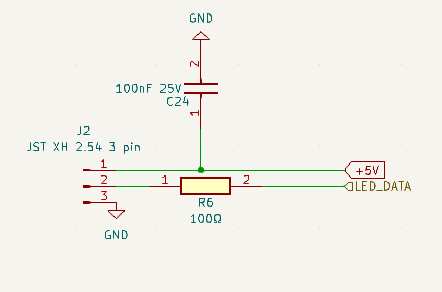
\includegraphics[width=0.8\textwidth]{LED.png}
    \caption{Schemat złącza paska LED}
    \label{fig:LED}
\end{figure}

\end{document}
